\documentclass{article}

\usepackage{tikz}
\usepackage{pgfplots}

\begin{document}

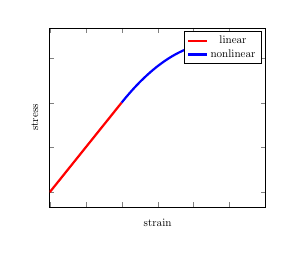
\begin{tikzpicture}[scale=0.4]
    \begin{axis}[
        xmin=0,
        xmax=3,
        xlabel=strain,
        ylabel=stress,
        xticklabels={,,},
        yticklabels={,,},
        domain=0:3,
        %legend style={at={(2.5,0.5)}, anchor=east}
        %legend pos=south east
    ]
    \addplot[red, line width=2pt] expression[domain=0:1,samples=40] {2*x};
    \addlegendentry{linear}
    % top of this parabola is at 7/3
    \addplot[blue, line width=2pt] expression[domain=1:7/3,samples=40] {-0.75*x*x+3.5*x-0.75};
    \addlegendentry{nonlinear}
    \end{axis}
\end{tikzpicture}

\end{document}
